\section{Die Monte-Carlo-Baumsuche}
\label{chap:mcts-intro}

Die Monte-Carlo-Baumsuche (engl.\ Monte Carlo Tree Search, MCTS) wurde 2006 von R\'{e}mi Coulom erstmals vorgestellt und im Go-Programm Crazy Stone mit großem Erfolg eingesetzt\autocite{coulomEfficientSelectivityBackup2007}.
Sie basiert auf der Kombination von Minimax-Spielbäumen mit Monte-Carlo-Simulationen.


\subsection{Spielbäume}
Ein Spiel kann formell mit den folgenden Elementen definiert werden\autocite[\ppno~162]{russellArtificialIntelligenceModern2009}:
\begin{itemize}
	\item $s_0$: Der \textbf{Ausgangszustand} des Spiels, zum Beispiel das leere Spielfeld
	\item $\textsc{Player}(s)$: Definiert welcher Spieler im Zustand $s$ am Zug ist
	\item $\textsc{Actions}(s)$: Definiert die Menge der legalen Spielzüge im Zustand $s$
	\item $\textsc{Transition}(s,a)$: Die \textbf{Übergangsfunktion} definiert den Folgezustand $s^\prime$, wenn Aktion $a$ im Zustand $s$ gewählt wurde
	\item $\textsc{Terminal-Test}(s)$: Ein Test ob das Spiel im Zustand $s$ vorüber ist oder nicht
	\item $\textsc{Utility}(s,p)$: Eine Bewertungsfunktion (engl.\ utility function) die einen numerischen Wert für einen terminalen Zustand $s$ und einen Spieler $p$ liefert. Der Wert ist typischerweise -1, 0 oder +1 für eine Niederlage, Unentschieden oder einen Sieg, kann aber auch 0, $+\frac{1}{2}$ und +1 sein.
\end{itemize}

Mit dem Ausgangszustand, der \textsc{Actions} Funktion und der \textsc{Transition} Funktion kann ein Spielbaum definiert werden.
Ein Spielbaum (siehe Abb.~\ref{fig:spielbaum}) ist ein Baum in dem jeder Knoten einen \textbf{Zustand} des Spiels repräsentiert.
Der Übergang von einem Knoten zu einem der \textbf{Kinder} ist ein \textbf{Zug}.
Die Anzahl der Kinder eines Knotens ist auch als \textbf{Verzweigungsfaktor} bekannt.
Der \textbf{Wurzelknoten} des Baumes ist der anfängliche Zustand des Spiels.
Knoten ohne Kinder, in denen keine weiteren Züge möglich sind, sind \textbf{terminale Knoten}.
Der Spielzustand in diesen terminalen Knoten kann bewertet werden um ein Spielergebnis zu erhalten.

\begin{figure}[hbt!]
	\centering
	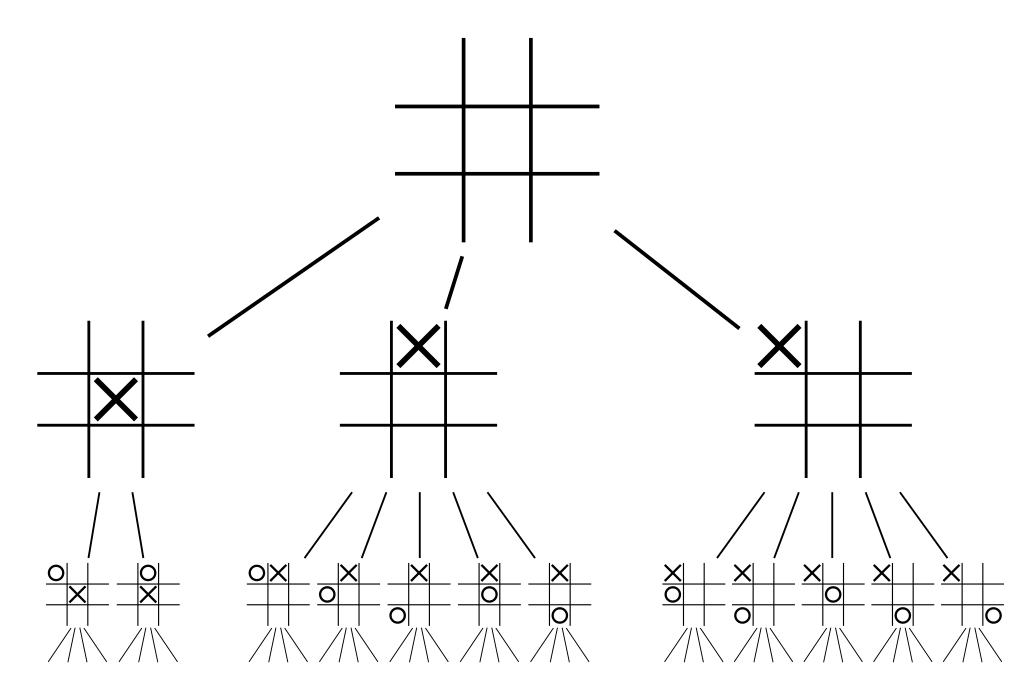
\includegraphics[width=0.7\linewidth]{1024px-Tic-tac-toe-game-tree}
	\caption[Ein Spielbaum mit den ersten zwei Zügen für Tic-Tac-Toe]{Ein Spielbaum mit den ersten zwei Zügen für Tic-Tac-Toe\protect\footnotemark}
	\label{fig:spielbaum}
\end{figure}

Spielbäume sind rekursive Datenstrukturen.
Wenn ein Zug gewählt wurde, kann der verbleibende Teilbaum, mit dem gewählten Folgezustand nun in der Wurzel, als neuer Spielbaum wiederverwendet werden.

Ein einfacher Algorithmus, der aber bei großen Spielbäumen aber schnell an seine Grenzen stößt, um den optimalen Spielzug in einem Spielbaum zu wählen ist der \textbf{Minimax-Algorithmus}. 

\label{chap:minimax}
In einem Zwei-Spieler-Nullsummenspiel sind die Ziele beider Spieler exakt entgegengesetzt.
Der eine Spieler versucht seinen (minimalen) Gewinn zu maximieren, während der Gegenspieler versucht, den (maximalen) Gewinn des ersten Spielers zu minimieren - daher der Name Minimax.
Dies spiegelt sich auch im Minimax-Spielbaum wieder indem es Max-Knoten und Min-Knoten gibt.
Bei Minimax wechseln sich die Knoten strikt ab, also Max-Knoten haben nur Min-Knoten als Kinder und umgekehrt.

\footnotetext{\cite{en:user:gdrFirstTwoPly2007}}

\medskip
\begin{figure}[hbt!]
	\centering
	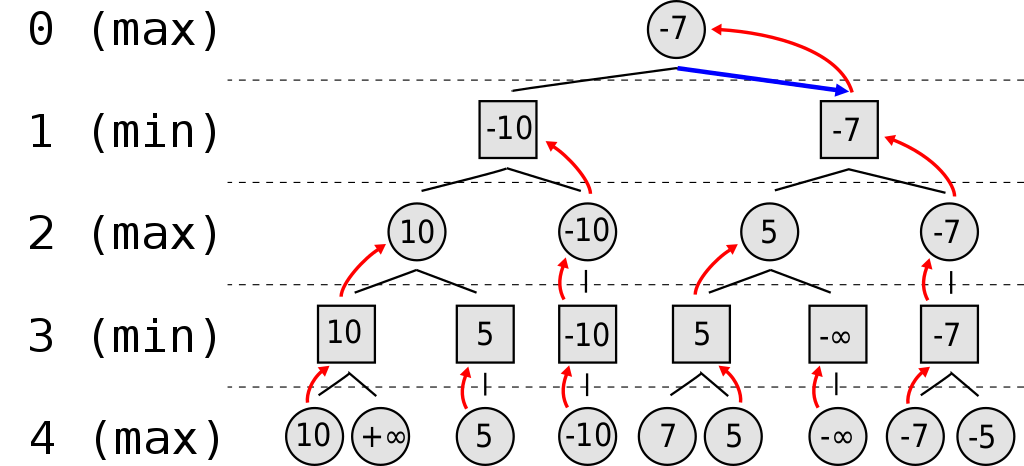
\includegraphics[width=0.7\linewidth]{1024px-Minimax}
	\caption[Minimax-Spielbaum]{Ein Minimax-Spielbaum mit Kreisen für Max-Knoten und Quadraten für Min-Knoten. Die roten Pfeile sind die gewählten Züge in jedem Knoten und der blaue Pfeil ist der gewählte Zug im Wurzelknoten. Die Zahlen in den Knoten stellen den Wert der Knoten dar. \protect\footnotemark }
	\label{fig:minimax}
\end{figure}
\footnotetext{\cite{nogueiraMinimaxAlgorithm2006}}

Minimax muss den gesamten Spielbaum erforschen, bis im Wurzelknoten ein optimaler Zug gewählt werden kann, da jeder Knoten von der Bewertung seiner Kindknoten abhängig ist.
Bei Spielen mit großem Verzweigungsfaktor wie Schach und Go führt dies aber zu gigantischen Spielbäumen, die einfach nicht komplett aufgebaut werden können.

Eine Lösung für dieses Problem ist es einfach die Suche ab einer gewissen Tiefe zu beenden und den aktuellen Zustand mit einer Bewertungsfunktion zu bewerten.
Dies hat sich aber zum Beispiel für Go als sehr schwierig herausgestellt, da es schwer ist eine angemessene Bewertungsfunktion zu definieren.

Die Alpha-Beta-Suche ist eine Modifikation der Minimax-Baumsuche, welche versucht nur so viel vom Spielbaum zu durchsuchen, wie es nötig ist.
Sobald festgestellt wird, dass ein weiteres Kind in einem Knoten das Ergebnis nicht verbessern kann, wird der gesamte Teilbaum "abgeschnitten" und nicht weiter berücksichtigt.


\subsection{Der MCTS-Algorithmus}
\label{chap:mcts-algo}
Coulom kombinierte erstmals die Erzeugung eines Spielbaumes mit Monte-Carlo Simulationen.
Unter Monte-Carlo Simulationen oder Monte-Carlo Experimenten versteht man gleichförmige Zufallsexperimente, die in großer Anzahl durchgeführt werden, um ein Ergebnis zu erhalten welches sich, mit steigender Anzahl der Experimente, dem tatsächlichen Wert immer weiter annähert.

Der von Coulom vorgestellt Algorithmus beginnt mit einem Knoten als Wurzel.
Ausgehend von diesem Wurzelknoten werden nun zufällige Simulationen des Spiels gespielt.
Das bedeutet in jedem Zustand wird ein zufälliger Zug gewählt und gespielt, bis das Spiel zu Ende ist.
Der erste Zustand in einer solchen Simulation, der sich noch nicht im Spielbaum befindet, wird zum Baum hinzugefügt.
Alle anderen Knoten, die sich bereits im Spielbaum befinden, merken sich, wie häufig sie bei solchen Simulationen besucht wurden und auch die Summe der Ergebnisse von Simulationen durch diesen Knoten.
Die gesammelten Statistiken werden dann bei nachfolgenden Simulationen benutzt, um vielversprechende Knoten häufiger zu besuchen.

\begin{figure}[hbt!]
	\centering
	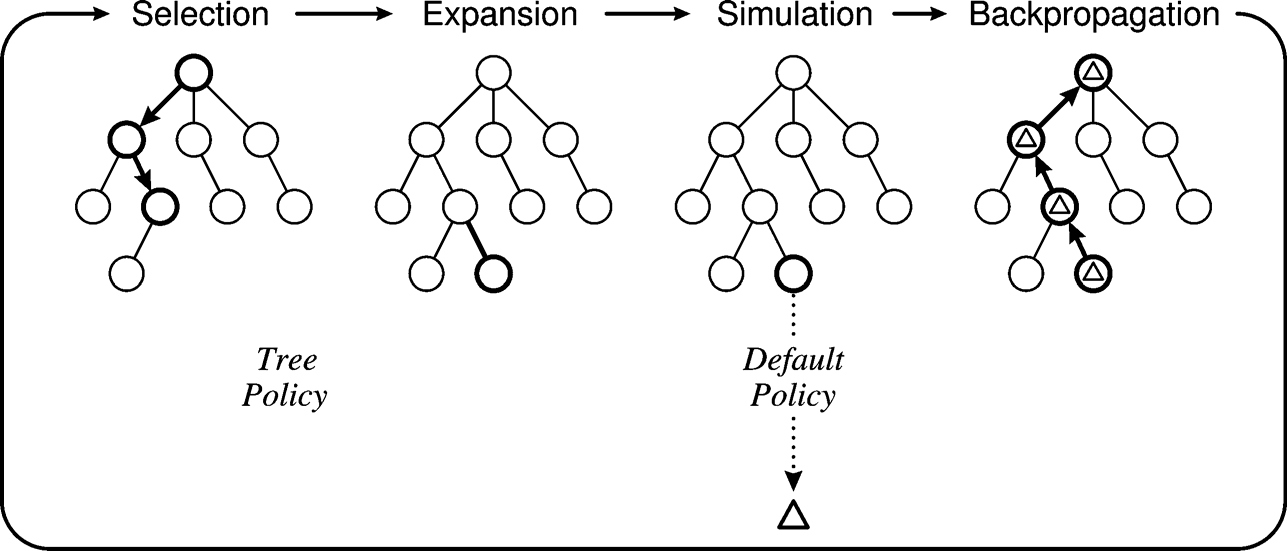
\includegraphics[width=0.7\linewidth]{mcts_survey_algorithm}
	\caption[Eine Iteration des MCTS Algorithmus]{Eine Iteration des MCTS Algorithmus\footnotemark}
	\label{fig:mctssurveyalgorithm}
\end{figure}
\footnotetext{\cite[\ppno~6]{browneSurveyMonteCarlo2012}}

Eine Iteration der Monte-Carlo-Baumsuche läuft in vier Schritten ab (siehe Abb.~\ref{fig:mctssurveyalgorithm}).
Zunächst wird der bestehende Spielbaum in einer \textbf{Selektions-Phase} durchlaufen, bis ein Blattknoten gefunden wurde.
Dabei folgt der Algorithmus eine bestimmten Strategie (engl. policy) um die Knoten im Baum zu wählen.
Ein Knoten ist ein Blatt des Baumes, wenn er terminal ist, oder noch nicht vollständig erforscht wurde, es also noch potentielle Kindknoten gibt, die noch nicht von diesem Knoten besucht wurden.
Wenn dieser Blattknoten nicht terminal ist, so wird er \textbf{expandiert} indem ein noch nicht besuchtes Kind hinzugefügt und besucht wird.
Ausgehend von diesem neuen Kindknoten wird nun eine \textbf{Simulation} gestartet.
Es werden so lange zufällige Spielzüge ausgewählt bis das Spiel einen Endzustand erreicht hat.
Die Strategie, die während der Simulation befolgt wird, nennt man auch die Default Policy.
In der Regel werden die Spielzüge zufällig gewählt, es können aber Heuristiken benutzt werden um die Simulation zu steuern.
Die Bewertung wird durch die Umgebung definiert, mit der der Algorithmus interagiert.
Dafür benötigt die MCTS eine sogenannte Forward-Simulation der Umgebung. Die Umgebung muss aus einem Zustand $s$ und einer Aktion $a$ einen Folgezustand $s^\prime$ und eine Belohnung $r$ erzeugen können. Das Ergebnis dieser Simulation wird dann in der \textbf{Backup-Phase} benutzt, um die Bewertungen der in der Selektion besuchten Knoten zu aktualisieren. Die Problemstellung bestimmt, ob es nur terminale Belohnungen gibt, also nur wenn die Simulation einen Endzustand erreicht hat, oder ob jeder einzelne Zustandsübergang eine Belohnung liefert.

Diese vier Schritte werden so lange wiederholt, bis ein Ressourcenlimit, zum Beispiel ein Zeitlimit, erreicht ist. Danach wird der beste Zug im Wurzelknoten ausgewählt. Die Expansion und Selektion lassen sich logisch noch zu einer Einheit als Tree Policy zusammenfassen.
Der Ablauf ist in Algorithmus \ref{algo:mcts} als Pseudocode erklärt. Das Programm geht von einem Spielzustand $s_0$ im Wurzelknoten $v_0$ aus. $\textsc{TreePolicy}$ folgt einer festen Strategie, um ein Blatt $v_l$ im Baum zu finden, welches dann expandiert wird, wenn es möglich ist. $\textsc{SimuliereSpiel}$ arbeitet mit dem Spielzustand im Blatt $s(v_l) = s_l$ und erzeugt daraus eine Bewertung $r$. Diese Bewertung wird durch $\textsc{Backup}$ vom Blatt bis zur Wurzel propagiert und aktualisiert die Statistiken in den Knoten. Nach Ablauf eines Zeitlimits wird mit $\textsc{BestesKind}$ der am besten bewertete Kindknoten im Wurzelknoten $v_0$ gewählt und die zugehörige Aktion $a(v)$ zurückgegeben.

\begin{algorithm}[H]
\begin{algorithmic}
\Function{MCTS}{$s_0$}
	\State $v_0\gets$ Knoten($s_0$)
	\While{noch Zeit übrig}
		\State $v_l\gets \Call{TreePolicy}{v_0}$
		\State $r\gets \Call{SimuliereSpiel}{s(v_l)}$
		\State $\Call{Backup}{v_l, r}$
	\EndWhile

\State \textbf{return} $a(\Call{BestesKind}{v_0})$
\EndFunction
\end{algorithmic}
\caption{Allgemeiner MCTS Algorithmus\footnotemark}
\label{algo:mcts}
\end{algorithm}
\footnotetext{\cite[\ppno~5]{browneSurveyMonteCarlo2012}}

\subsection{Upper Confidence Bounds applied to Trees (UCT)}

Parallel zur Arbeit von Coulom haben Kocsis und Szepesv\'{a}ri 2006 den \textbf{Upper Confidence Bounds applied to trees} (UCT)-Algorithmus \autocite{kocsisBanditBasedMonteCarlo2006} entwickelt. UCT gilt heute als beliebtester MCTS-Algorithmus. Die Besonderheit von UCT liegt in seiner Tree Policy und damit in der Art, wie die Knoten im Baum ausgewählt werden. Kocsis und Szepesv\'{a}ri betrachten dabei die Auswahl eines Kindknotens als ein sogenanntes Banditenproblem. \autocite[\ppno~25\psqq]{suttonReinforcementLearningIntroduction2018}

\bigskip
Banditenprobleme sind eine Klasse von Problemen im bestärkenden Lernen, in denen der Agent zu jedem Zeitschritt $t$ aus $K$ Optionen wählen muss, um eine kumulative Belohnung zu maximieren, indem die optimale Aktion so oft wie möglich gewählt wird. Die Verteilung der Belohnungen jeder Aktion ist unbekannt aber statisch und die Belohnungen aus sukzessiven Aktionen sind voneinander unabhängig. Der Agent muss lernen, nur durch gesammelte Erfahrung seine erhaltene Belohnung auf lange Sicht zu maximieren. Verhält er sich gierig und wählt nur die Aktion mit der höchsten durchschnittlichen Belohnung, so werden alle Aktionen ignoriert, die im ersten Versuch keine Belohnung geliefert haben. Verbringt er dagegen zu viel Zeit damit, andere Aktionen als die derzeit beste zu erforschen, wählt er häufig suboptimale Aktionen. 

Dieses Problem, auch bekannt als \textbf{exploration-exploitation-Dilemma}, ist ein Grundproblem vieler Algorithmen des bestärkenden Lernens. Die beste Strategie für das Banditenproblem ist die upper confidence bound (UCB) Regel \textbf{UCB1} von Auer et.al \autocite[\ppno~237]{auerFinitetimeAnalysisMultiarmed2002}. Der Agent wählt die Aktion $j, 1 \le j \le K$, die die Gleichung

\begin{equation}
\bar{X}_j + \sqrt{\frac{2\ln n}{n_j}}
\label{eqn:UCB1}
\end{equation}

maximiert. Wobei $\bar{X}_j$ die durchschnittliche Belohnung ist, die bisher durch das Spielen von Aktion $j$ erhalten wurde, $n_j$ ist die Anzahl der Spielzüge in denen $j$ gewählt wurde und $n$ ist die Anzahl der insgesamt gespielten Spielzüge. Diese Gleichung besteht aus einem exploitation-Teil $\bar{X}_j$ und einem exploration-Teil $\sqrt{\frac{2\ln n}{n_j}}$. Der exploration-Teil repräsentiert die Unsicherheit in der Bewertung der Aktion $j$. Wenn die Aktion noch nicht oft gewählt wurde, $n_j$ also im Vergleich zu $n$ gering ist, so wird dieser Teil größer. Die Bewertung $\bar{X}_j$ ist noch sehr unsicher. Wurde dagegen $j$ sehr häufig gewählt, so wird der exploration-Teil kleiner und somit drücken wir eine hohe Sicherheit in der Schätzung des Wertes $\bar{X}_j$ aus.

\bigskip
Im UCT-Algorithmus wird die Auswahl des Kindknotens zu einem Banditenproblem. Dafür hat jeder Knoten $v$ eine Statistik $Q(v)$ mit der insgesamt erhaltene Belohnung in diesem Knoten und $N(v)$ mit der Anzahl der Besuche des Knotens. Das gewählte Kind ist dann jenes, welches die Formel

\begin{equation}
UCT = \frac{Q(v^\prime)}{N(v^ \prime)} + C_p\sqrt{\frac{\ln N(v)}{N(v^\prime)}}
\label{eqn:UCT}
\end{equation}

maximiert. Der Faktor $\sqrt{2}$ wurde aus der ursprünglichen UCB1-Formel (\ref{eqn:UCB1}) herausgezogen und als Parameter $C_p$ variierbar gemacht. Er kann für jedes Problem optimiert werden und bestimme Verbesserungen funktionieren besser mit verschiedenen Werten von $C_p$. Algorithmus \ref{algo:UCT} zeigt den vollen Pseudocode des UCT Algorithmus.

\begin{algorithm}[H]
\begin{algorithmic}[1]
\Function{UCT}{$s_0$}
	\State $v_0\gets$ Knoten($s_0$)
	\While{noch Zeit übrig}
		\State $v_l\gets$ \Call{TreePolicy}{$v_0$}
		\State $r\gets$ \Call{SimuliereSpiel}{$s(v_l)$}
		\State \Call{Backup}{$v_l, r$}
	\EndWhile 
	
\State \textbf{return} $a(\Call{BestesKind}{v_0,0})$
\EndFunction

\Function{TreePolicy}{$v$}
	\While{$v$ ist nicht terminal}
		\If{$v$ ist nicht vollständig expandiert}
			\State \textbf{return} \Call{Expandiere}{$v$}
		\Else
			\State $v \gets \textsc{BestesKind}(v)$
		\EndIf
	\EndWhile
	 
	\State \textbf{return} $v$
\EndFunction

\Function{Expandiere}{$v$}
	\State wähle $a \in$ noch nicht gewählte Aktionen aus $A(s(v))$
	\State füge ein neues Kind $v^\prime$ zu $v$ hinzu
	\State mit $s(v^\prime) = \textsc{Transition}(s(v),a)$
		\State und $a(v^\prime) = a$
		\State \textbf{return} $v^\prime$
\EndFunction

\Function{BestesKind}{$v, C_p$}\\
\State \textbf{return} $\argmax_{v^\prime \in\ \text{Kinder von}\ v} \frac{Q(v^\prime)}{N(v^\prime)} + C_p \sqrt{\frac{\ln N(v)}{N(v^\prime)}}$
\EndFunction

\Function{SimuliereSpiel}{$s$}
\While{$s$ ist nicht terminal}
\State wähle $a \in A(s)$ zufällig
\State $s \gets \textsc{Transition}(s,a)$
\EndWhile

\State \textbf{return} Belohnung für $s$
\EndFunction
\end{algorithmic}
\caption{Upper Confidence Bound applied to Trees\footnotemark}
\label{algo:UCT}
\end{algorithm}
\footnotetext{\cite[\ppno~7\psq]{browneSurveyMonteCarlo2012}}

Zusätzlich zu $Q(v)$ und $N(v)$ enthalten die Knoten noch Informationen über ihren Spielzustand $s(v)$ und die Aktion die in den Knoten geführt hat $a(v)$ sowie ein Verweis auf den Elternknoten. Die Backup-Regel ist unterschiedlich definiert für Ein-Spieler-Spiele und für Zwei-Spieler-Nullsummenspiele. Für Zwei-Spieler-Spiele in denen die Belohnungen für Spieler 1 gegenteilig zu den Belohnungen für Spieler 2 sind - $+1$ für Spieler 1 bedeutet $-1$ für Spieler 2 - kann die Belohnung des anderen Spielers durch Negierung in jedem Backup-Schritt erhalten werden.


\begin{algorithm}[H]
\begin{algorithmic}		
\Function{Backup}{$v, r$} \Comment{Ein-Spieler Backup}
	\While{$v$ ist nicht null}
		\State $N(v) \gets N(v) + 1$
		\State $Q(v) \gets Q(v) + r$
		\State $v \gets \text{Elternknoten von}\ v$
	\EndWhile
\EndFunction\\

\Function{Backup}{$v, r$} \Comment{Minimax Backup}
	\While{$v$ ist nicht null}
		\State $N(v) \gets N(v) + 1$
		\State $Q(v) \gets Q(v) + r$
		\State $r \gets -r$
		\State $v \gets \text{Elternknoten von}\ v$
	\EndWhile
\EndFunction
\end{algorithmic}
\caption{Backup-Regeln für Ein-Spieler und Zwei-Spieler Minimax}
\end{algorithm}

Dieser normale UCT (engl. plain UCT) Algorithmus, wie er von Kocsis und Szepesv\'{a}ri vorgestellt wurde, wird in Kapitel \ref{chap:mcts-impl} implementiert und als Ausgangslage für alle weiteren Verbesserungen genommen. 

\subsection{Verbesserungen}

Die verschiedenen Schritte der Baumsuche können verändert und verbessert werden und werden dadurch besser für die jeweiligen Anwendungsfälle geeignet. Im Paper "A survey of monte carlo methods" von Browne u.a.\autocite{browneSurveyMonteCarlo2012} wird eine große Menge von Verbesserungen vorgestellt und eine Übersicht darüber gegeben, für welche klassischen Spiele sie nützlich sein könnten. Im folgenden werde ich eine Handvoll ausgewählter Verbesserungen vorstellen.

\subsubsection{Transpositionen}
\label{transpos}
Unter Transpositionen versteht man identische Spielzustände, die über unterschiedliche Zugkombinationen erreicht werden. Ein solcher Spielzustand wird zum Beispiel über die Zugfolge d1,e1;c1,d2 erreicht (Abb. \ref{fig:c4transpos}).

\begin{figure}[hbt!]
	\centering
	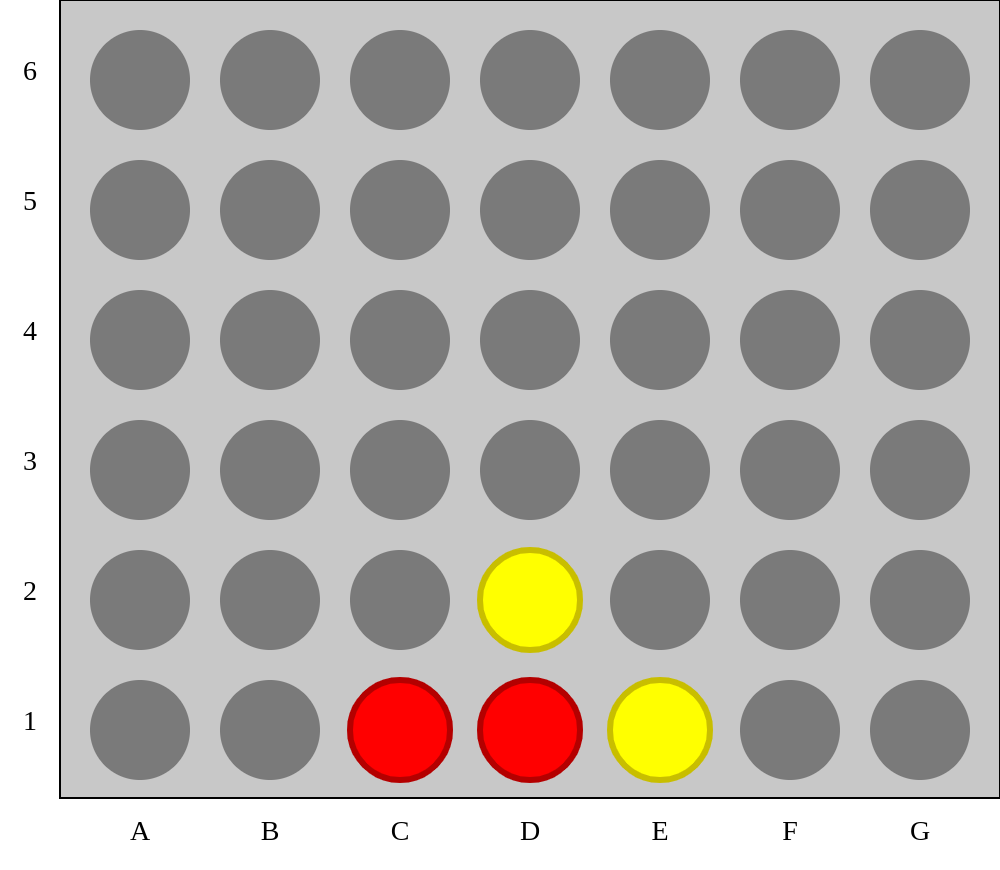
\includegraphics[width=0.7\linewidth]{c4_transpos}
	\caption[Transposition in Vier Gewinnt]{Die Spielposition kann auf mehrere Wegen erreicht werden. Die Züge d1,e1;c1,d2 sowie d1,d2;c1,e1 und c1,e1;d1,d2 führen alle zum selben Ergebnis.}
	\label{fig:c4transpos}
\end{figure}

Eine andere Zugfolge, die zum selben Spielzustand führt, ist d1,d2;c1,e1. Durch diese unterschiedlichen Pfade werden die beiden identischen Zustände normalerweise als separate Knoten mit separaten Statistiken gespeichert. Es würde aber sehr viel Sinn ergeben, diese Knoten zu kombinieren, denn der Weg, wie ein Zustand erreicht wird, hat keinen Einfluss darauf, welches die beste Aktion in diesem Zustand ist. Childs u.a. schlagen in ihrem Paper "Transpositions and Move Groups in Monte Carlo Tree Search"\autocite[\ppno~390\psq]{childsTranspositionsMoveGroups2008} drei Anpassungen des UCT-Algorithmus vor, um mit Transpositionen umzugehen. 

Normale UCT-Algorithmen, die Transpositionen nicht berücksichtigen, werden im Paper als \textbf{UCT0} bezeichnet. 

In Gleichung \ref{eqn:UCT} verwende ich die Statistiken eines Knotens $Q(v)$ und $N(v)$ direkt, also die Summe der Belohnungen aus Simulationen und die Anzahl an Simulationen durch diesen Knoten. Zusätzlich dazu kann diese Statistik abhängig von der gewählten Aktion $a$ im Knoten $v$, $Q(v,a)$ und $N(v,a)$ gespeichert werden. Wenn keine Transpositionen identifiziert werden, so sind die Werte identisch $v^\prime = \textsc{Transition}(s(v),a) \Rightarrow Q(v^\prime) = Q(v,a)$. Werden Transpositionen aber erkannt, kann es mehrere Aktionen in verschiedenen Knoten geben, die zum selben Kindknoten führen.

Wenn Transpositionen erkannt werden, so können sich im einfachsten Fall die Knoten, unabhängig davon wo sie sich im Baum befinden, ihre Statistiken teilen. Dies hat vor allem den Vorteil, dass der gesamte Baum kleiner wird. Die von Childs u.a. vorgeschlagene einfache Auswahlregel UCT1 ist:

\begin{equation}
UCT1 = \argmax_{a \in A(v)} \frac{Q(v,a)}{N(v,a)} + C_p\sqrt{\frac{\ln N(v)}{N(v,a)}}
\label{eqn:UCT1}
\end{equation}

Diese unterscheidet zwischen den verschiedenen Wegen, die zum selben Knoten geführt haben können, kumuliert aber die Statistiken von Knoten mit identischen Zuständen. Die zweite Vorgeschlagene Auswahlregel macht Gebrauch von mehr Informationen aus den Transpositionen, indem statt der Bewertung der Aktion $Q(v,a)$ die Bewertung des Folgezustands $Q(v^\prime)$ wie in der originalen UCT Implementierung verwendet wird (siehe Gleichung\~\ref{eqn:uct2}). Für die Berechnung des Erkundungsfaktors wird weiterhin $N(v,a)$ anstatt $N(v^\prime)$ im Nenner benutzt, da laut Childs die Auswahl sonst nicht mehr auf den korrekten Knoten konvergiert, wenn der der Knoten $v^\prime$ sehr häufig über einen anderen Pfad besucht wurde.

\begin{equation}
UCT2 = \argmax_{a \in A(v)} \frac{Q(v^\prime)}{N(v^\prime)} + C_p\sqrt{\frac{\ln N(v)}{N(v,a)}}
\label{eqn:UCT2}
\end{equation}

Die letzte vorgeschlagene Variante berechnet den Wert der Kinder $Q(v^\prime)$ rekursiv als gewichteter Durschnitt aller Kinder dieses Kindknotens. Dadurch, dass rekursiv alle Kinder eines Knotens betrachtet werden müssen, ist der Rechenaufwand in der Methode \textsc{bestesKind} sehr hoch. Um ihn zu reduzieren, können die Durchschnittswerte in den Knoten zwischengespeichert werden und müssen sich nur ändern, wenn sich ein Kind verändert. Damit kann der Rechenaufwand aus der teuren Selektionsphase in die Backupphase verlagert werden.

%TODO: UCT3 Gleichung
\begin{equation}
UCT3 = \argmax_{a \in A(v)}
\label{eqn:uct3}
\end{equation}

Durch das Kombinieren der Knoten entsteht ein gerichteter azyklischer Graph. Es kann nützlich sein, zur Bewertung eines Knotens nicht nur die direkten Kinder und Eltern zu betrachten, sondern beliebig tief im Graph auf- und abzusteigen. Cazenave, Mehat und Saffidine schlagen einen parametrisierbaren UCT Algorithmus, den sie Upper confidence bound for rooted directed acyclic graphs (UCD) nennen, vor. Sie zeigen wie mit dieser Parametrisierung die UCT1-3 Algorithmen von Childs u.a. implementiert werden können. Cazenave u.a. argumentieren dafür, die Statistiken nicht in den Knoten sondern in den Kanten zu speichern, dies kann allerdings die Implementierung verkomplizieren und wird deshalb bei der Anwendung von Transpositionen eher selten umgesetzt.
Der UCD-Algorithmus besteht aus drei Komponenten.
%TODO: UCD Gleichungen und Quelle
\begin{equation}
Gleichung1
\label{eqn:ucd1}
\end{equation}
\begin{equation}
Gleichung2
\label{eqn:ucd2}
\end{equation}
\begin{equation}
Gleichung3
\label{eqn:ucd3}
\end{equation}


\subsubsection{Score Bounded MCTS}
\label{chap:scorebounded}
%TODO: Referenz Alpha-Beta Cuts, Scorebounded Quelle
Score Bounded MCTS ist konzeptionell ähnlich zu Alpha-Beta Cuts im Minimax-Suchalgorithmus.
Jeder Knoten speichert eine optimistische $opt(v)$ und pessimistische Grenze $pess(v)$ für seine Kindknoten.
Die Bewertung hängt davon ab, ob der Knoten ein Min- oder ein Max-Knoten (siehe Seite~\ref{chap:minimax}) ist.
Für einen Max-Knoten werden die optimistischsten, also die maximalen, Werte der Kinder genommen.
Das heißt $opti(v) = \max_{k \in\ \text{Kinder von}\ v}opti(k)$ und $pess(v) = \max_{k \in\ \text{Kinder von}\ v}pess(k)$.
Ein Min-Knoten dagegen nimmt die minimalen Werte der Kinder $opti(v) = \min_{k \in\ \text{Kinder von}\ v}opti(k)$ und $pess(v) = \min_{k \in\ \text{Kinder von}\ v}pess(k)$.
Wenn ein Knoten terminal ist, so gilt $pess(v) = opti(v) = \textsc{Utility}(s(v),P_{max})$, die Grenzen entsprechen also der tatsächlichen Bewertung des Zustands durch die Umgebung aus Sicht des Max-Spielers. Der Einfachheit halber sind die Grenzen auch in einem Minimax-Baum immer aus Sicht des Max-Spielers definiert, das heißt bei terminalen Bewertungen von $[-1, 0, 1]$ für Niederlage, Unentschieden und Sieg ist ein Knoten mit $pess(v) = opti(v) = 1$ immer gut für den Max-Spieler respektive $pess(v) = opti(v) = -1$ ist immer schlecht für Max. Die Grenzen werden initialisiert mit $pess(v) = \textsc{Niederlage}$, $opti(v) = \textsc{Sieg}$ und erst aktualisiert, wenn ein Endzustand \textbf{im Baum} erreicht wurde, also ein terminaler Blatt-Knoten dem Baum hinzugefügt wurde.
Erst dann ist die tatsächliche Bewertung eines Knotens bekannt.

Die Grenzen können benutzt werden um Teile des Suchbaumes zu ignorieren, wenn durch die Grenzen bekannt ist, dass dieser Teilbaum die Bewertung nicht weiter verbessern kann, der Baum wird "beschnitten" (engl.\ pruned).
In einem Max-Knoten (bzw.\ Min-Knoten) $n$ kann der Kindknoten $s$ ignoriert werden, wenn $opti(s) \le pess(n)$ ($pess(s) \ge opti(n)$).\cite[\ppno~5]{cazenaveScoreBoundedMonteCarlo2011}

Zusätzlich zum Beschneiden des Baumes können die Grenzen benutzt werden, um die Selektion zu beeinflussen.
So können zum Beispiel Knoten mit einer hohen optimistischer Grenze bevorzugt besucht werden, während versucht wird Knoten mit geringer pessimistischer Grenze zu vermeiden.
Zum Beispiel

\begin{equation}
Q_sb(v) = \frac{Q(v)}{N(v)} + \gamma opti(v) + \delta pess(v)
\label{eqn:scorebound}
\end{equation}

mit $-1 \le \gamma, \delta \le 1$.

Da die Grenzen eines Knotens von den Grenzen der Kindknoten abhängig ist, ist es notwendig die Grenzen so selten wie möglich zu aktualisieren und nicht bei jeder Iteration der Baumsuche neu zu berechnen.
Dafür schlagen Cazenave und Saffidine zwei einfache Algorithmen vor, die die Grenzen aus einem terminalen Knoten effizient den gesamten Baum hinaufpropagieren.


\begin{algorithm}[H]
\begin{algorithmic}
\Function{prop_pess}{$s$}
	\If{$s$ ist nicht die Wurzel}
		\State $n \gets \text{Elternknoten von }s$
		\State old\_pess \gets $pess(n)$
		\If{old\_pess < $pess(s)$}
			\If{$n$ ist ein Max Knoten}
				\State $pess(n) \gets pess(s)$
				\Call{prop_press}{$n$}
			\Else
				\State $pess(n) \ gets \min_{s' \in children(n)}pess(s')$
				\If{old\_pess > $pess(n)$}
					\Call{prop_press}{$n$}
				\EndIf
			\EndIf
		\EndIf
	\EndIf
\EndFunction


\Function{prop_opti}{$s$}
	\If{$s$ ist nicht die Wurzel}
		\State $n \gets \text{Elternknoten von }s$
		\State old\_opti \gets $opti(n)$
		\If{old\_opti > $opti(s)$}
			\If{$n$ ist ein Max Knoten}
				\State $opti(n) \gets \max_{s' \in children(n)}opti(s')$
				\If{old_opti > $opti(n)$}
					\Call{prop_opti}{$n$}
				\EndIf
			\Else
				\State $opti(n) \gets opti(s)$
				\Call{prop_opti}{$n$}
			\EndIf
		\EndIf
	\EndIf
\EndFunction
\end{algorithmic}
\caption{Algorithmus zur Aktualisierung der pessimistischen und optimistischen Grenzen.\footnotemark}
\label{algo:prop-scorebound}
\end{algorithm}
\footnotetext{\cite[\ppno~4]{cazenaveScoreBoundedMonteCarlo2011}}

\subsubsection{Rapid Action Value Estimation}

Rapid Action Value Estimation (RAVE) gehört zur Gruppe der All Moves as First (AMAF)-Verbesserungen.
In der regulären Monte-Carlo-Baumsuche werden nur die tatsächlich besuchten Knoten in der Backup-Phase aktualisiert.
Anstatt die besuchten Knoten und damit die konkreten Zustände zu betrachten, berücksichtigt die All Moves as First Verbesserung die gemachten Spiel\textbf{züge}. Der Gedanke dahinter ist, dass ein Spielzug $A$ der im Zustand $s_1$ gemacht wurde, in den Zuständen $s_t, t > 1$ genauso oder ähnlich gut ist. Im Schach ist zum Beispiel ein Zug, in dem ein Bauer eine stärkere Figur schlägt, (fast) immer gut, egal wie das restliche Spielfeld aussieht.

%TODO: Quelle für RAVE
Die verschiedenen AMAF-Verfahren unterscheiden sich dadurch, wie sie dieses Wissen speichern und verwenden. Manche verfahren aktualisieren die Statistik $Q(v)$ direkt, andere führen separate AMAF-Statistiken, um sie später gewichtet zu kombinieren. RAVE speichert die AMAF-Statistik $Q_RAVE(v)$ und $N_RAVE(v)$ separat und verwendet sie in der Selektionsphase bei der Auswahl der Kindknoten. Die Kombination der RAVE-Statistik mit der regulären MCTS-Statistik wird durch einen Parameter $\beta$ gesteuert.

\begin{equation}
UCT_{RAVE}=\beta * \frac{Q_RAVE(v^\prime)}{N_RAVE(v^\prime)} + (1-\beta) * \frac{Q(v^\prime)}{N(v^\prime)} + C_p * \sqrt{\frac{\ln(N(v))}{N(v^\prime)}}
\label{eqn:uct-rave}
\end{equation}

\begin{equation}
\beta = \frac{N_{RAVE}(v^\prime)}{N(v^\prime)+N_{RAVE}(v^\prime)+N(v^\prime)*N_{RAVE}(v^\prime)*b^2}
\label{eqn:beta}
\end{equation}


Wenn dieser Parameter während der gesamten Baumsuche konstant bleibt, so nennt man diesen Algorithmus auch $\alpha$-AMAF, mit einem konstanten $\alpha \in [0,1]$. Das besondere an RAVE ist, dass sich dieser Parameter im Laufe der Baumsuche verändert. Wenn ein Knoten noch wenig besucht wurde, so ist $\beta$ nahe $1$, wodurch fast ausschließlich die RAVE-Statistik benutzt wird. Mit mehr Besuchen der Kindknoten, wird die gesammelte Statistik $Q(v)$ genauer und somit kann ein niedrigerer Wert für $\beta$ verwendet werden. Der Hyperparameter $b$ in Gleichung \ref{eqn:beta} kann angepasst werden, um RAVE gezielter anzupassn.

In der Selektions- und Simulations-Phase wird eine Liste aller gemachten Spielzüge geführt. Beim Backup werden dann auch alle Nachbarknoten im Baum aktualisiert, die durch einen der, später in der Simulation gemachten, Spielzüge erreicht werden könnten.

Was in der Literatur nicht erwähnt wird, ist die Notwendigkeit die Spielzüge eindeutig zu identifizieren. Die meisten Untersuchungen des Algorithmus beziehen sich nur auf Schach und Go, in denen ein Spielzug klar definiert ist (schwarzer Bauer von E2 nach E3 oder schwarzer Stein auf Kreuzung 3,3).
Für Vier Gewinnt reicht es nicht, dass Spieler 1 einen Stein in Spalte 4 setzt, denn der tatsächlich resultierende Zug hängt davon ab, wie viele Steine sich bereits in der Spalte befinden. Darum muss jeder Zugname in Vier Gewinnt Informationen über den agierenden Spieler, die Spalte und die Zeile im Spielbrett enthalten.

